\clearpage
\section{Appendix C}
\label{apx:mediaRecipies}

\begin{itemize}
    \item \textbf{\Acf{pdb}}: 24g potato dextrose (Sigma-Aldrich, UK) per L of distilled water.
    \item \textbf{\Acf{pda}}: 24g potato dextrose (Sigma-Aldrich, UK)  and 15g of agar (Sigma-Aldrich, UK) per L of distilled water.  
    \item \textbf{\Acf{ypgb}}: 5g yeast extract (Sigma-Aldrich, UK), 5g peptone (Sigma-Aldrich, UK), and 10g glucose  (Sigma-Aldrich, UK) per L of distilled water. 
    \item \textbf{\Acf{ypgb}}: 5g yeast extract (Sigma-Aldrich, UK), 5g peptone (Sigma-Aldrich, UK), 10g glucose (Sigma-Aldrich, UK), and 15g agar (Sigma-Aldrich, UK) per L of distilled water.
\end{itemize}

\newpage
\label{apx:outliers}

\begin{figure}[hp!]
    \centering
    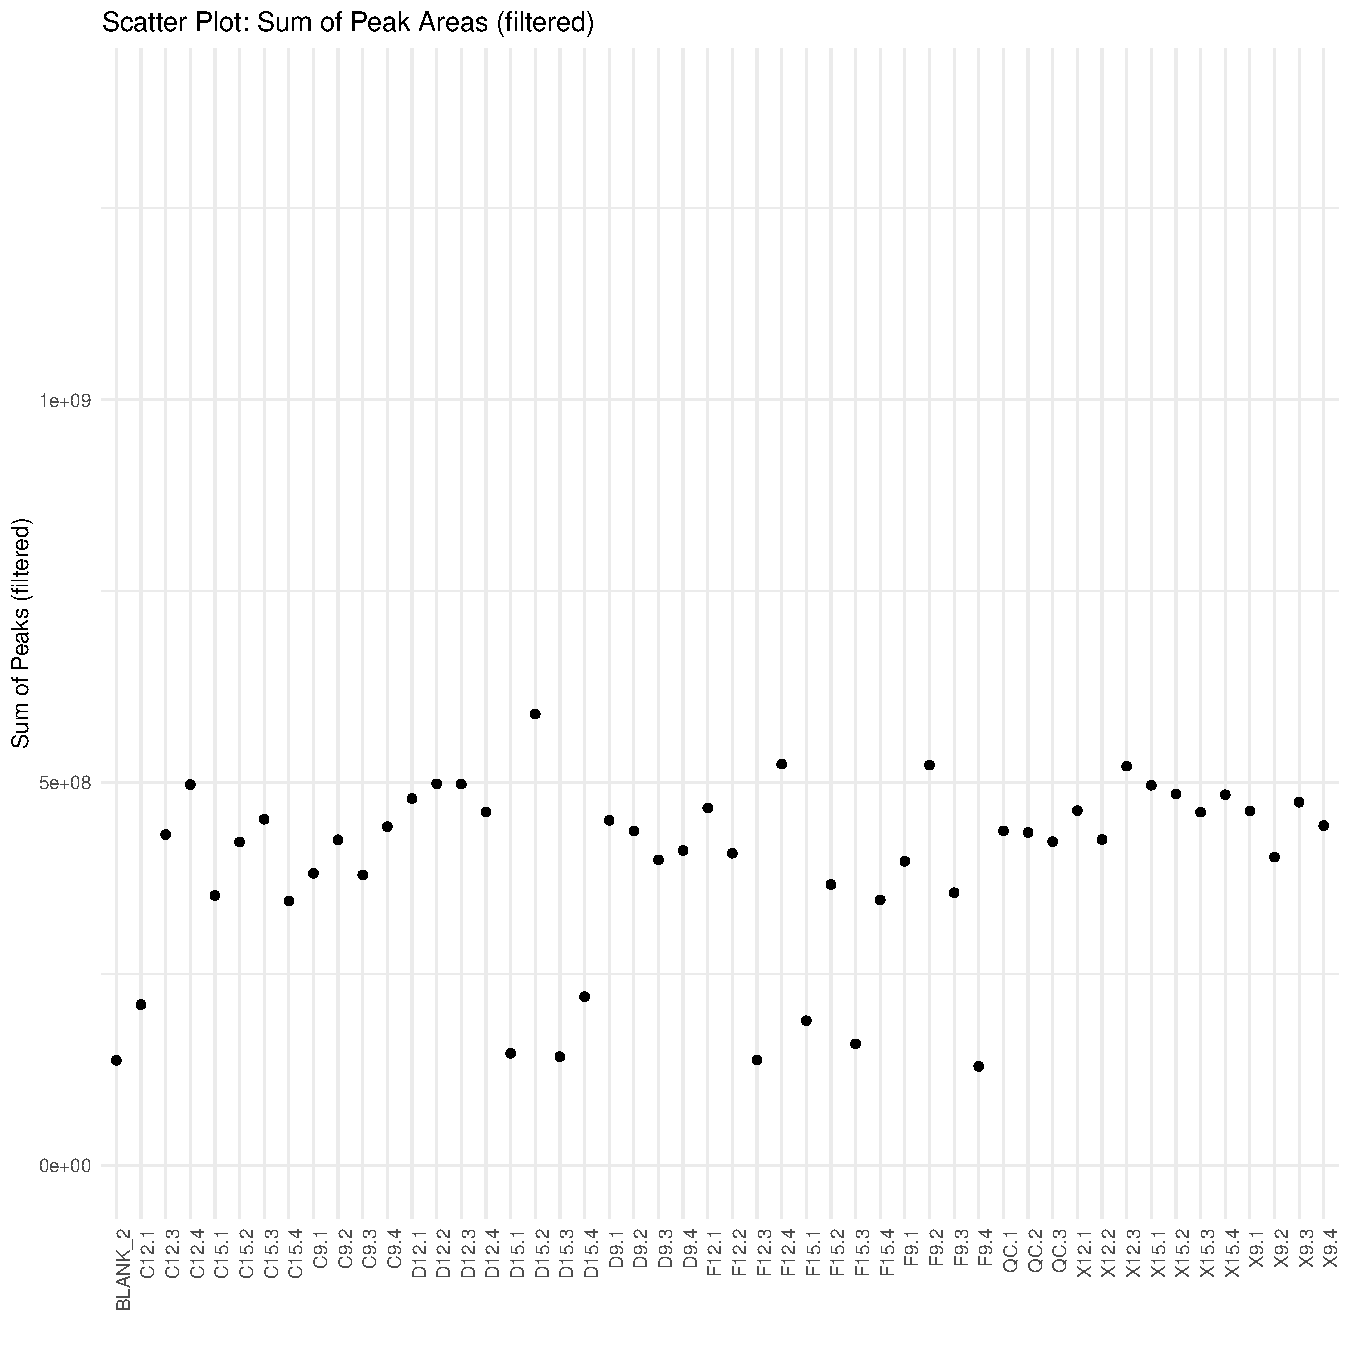
\includegraphics[width=\textwidth]{Appendices/sum_plot-filtered.pdf}
    \caption[Outliers identified in the dataset] {\textbf{Outliers identified in the dataset.} The sum of all features across samples. Samples C12.1, D15.1, D15.3, D15.4, F12.3, F15.1, F15.3, and F9.4 were identified as outliers and removed from the dataset. The blank samples were also removed from the statistical analysis.} 
    \label{fig:SampleSumPlot}
\end{figure}

\begin{figure}[htp!]
    \centering
    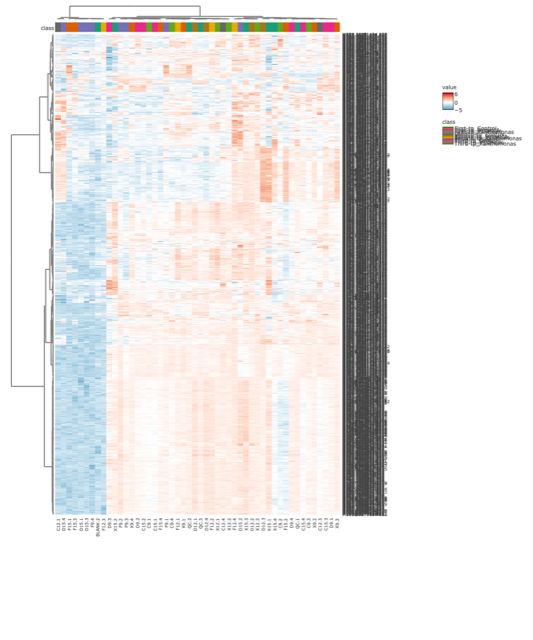
\includegraphics[width=\textwidth]{Figures/AllFeaturesAllSamples_Clustered.png}
    \caption[Heatmap showing hierarchical clustering of samples based on feature peak intensities.]{\textbf{Heatmap showing hierarchical clustering of samples based on 3931 feature peak intensities.} The distance measure was Euclidean and the ward.D algorithm was used for clustering. Class shows the treatment time and group. Value shows the normalised peak intensity. Values show normalised peak intensity. Features were normalised to the sodium formate \ch{Na(NaCOOH)3} adduct ($m/z=226.9521$), log-transformed and scaled (Pareto scaling). Figure generated using MetaboAnalyst (v6.0).}
    \label{fig:AllFeaturesAllSamples}
\end{figure}



\begin{figure}[ph!]
  \centering
  \begin{subfigure}[b]{\textwidth}
    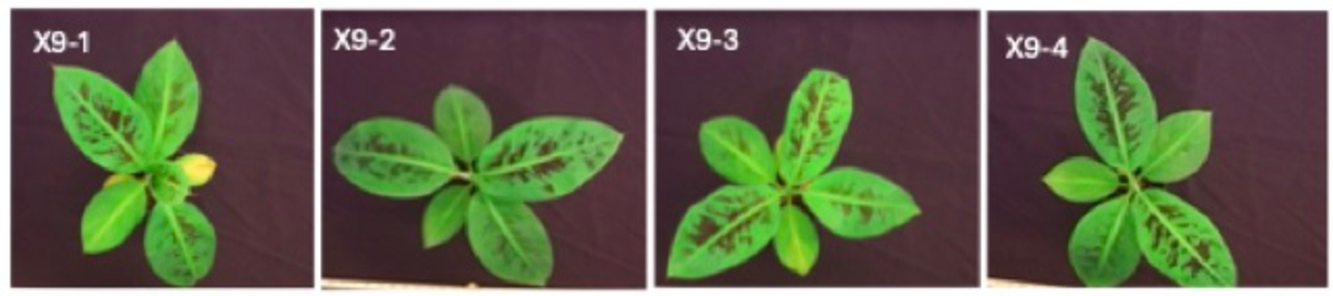
\includegraphics[width=\textwidth]{Figures/FirstTimePointXanthomonasBLQs.pdf}
    \caption{}
    \label{fig:XvmFirstTimeBLQs}
  \end{subfigure}
   \begin{subfigure}[b]{\textwidth}
    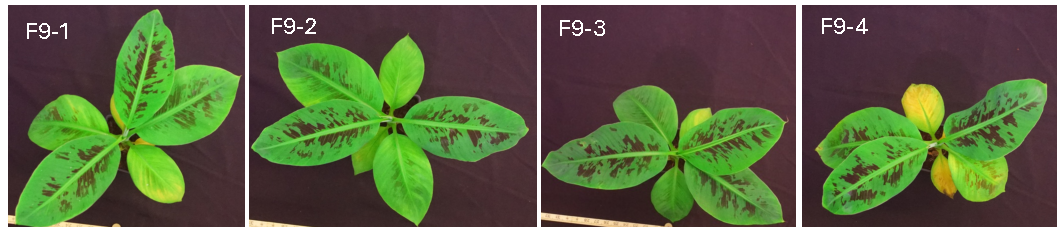
\includegraphics[width=\textwidth]{Figures/FirstTimePointFusariumBLQs.pdf}
    \caption{}
    \label{fig:FocFirstTimeBLQs}
  \end{subfigure}
     \begin{subfigure}[b]{\textwidth}
    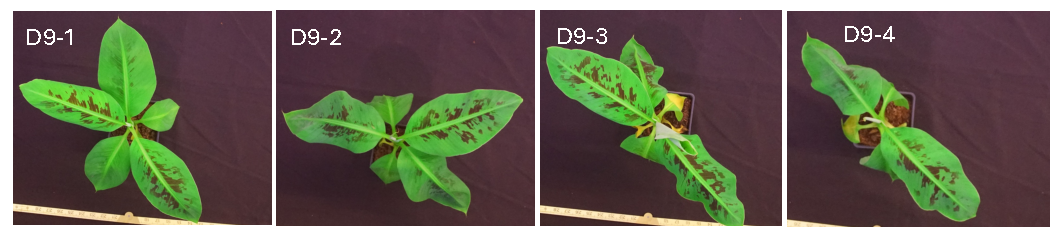
\includegraphics[width=\textwidth]{Figures/FirstTimePointDroughtBLQs.pdf}
    \caption{}
    \label{fig:DroFirstTimeBLQs}
  \end{subfigure}
     \begin{subfigure}[b]{\textwidth}
    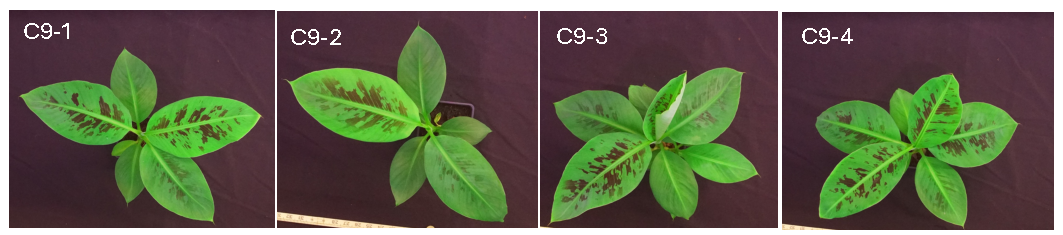
\includegraphics[width=\textwidth]{Figures/FirstTimePointControlBLQs.pdf}
    \caption{}
    \label{fig:ConFirstTimeBLQs}
  \end{subfigure}
  \caption[RGB images of 'Grande Naine' banana plants at the first sample time points.]{\textbf{RGB images of 'Grande Naine' banana plants at the first sample time points.}
  \textbf{\subref{fig:XvmFirstTimeBLQs}}) \acl{xvm}-inoculated plants at 7 \acl{dpi}.
  \textbf{\subref{fig:FocFirstTimeBLQs}}) \acl{Focub4}-inoculated plants at 15 \acl{dpi}.
  \textbf{\subref{fig:DroFirstTimeBLQs}}) Drought-stressed plants at 7 \ac{dpi}, no-watering.
  \textbf{\subref{fig:ConFirstTimeBLQs}}) Mock-inoculated plants at 7 \ac{dpi}.
  Plant labels are provided in white text and correspond to sample labels used in \acl{um} analysis.
  }
  \label{fig:FirstTimePointSymptoms}
\end{figure}

\begin{figure}[ph!]
  \centering
  \begin{subfigure}[b]{\textwidth}
    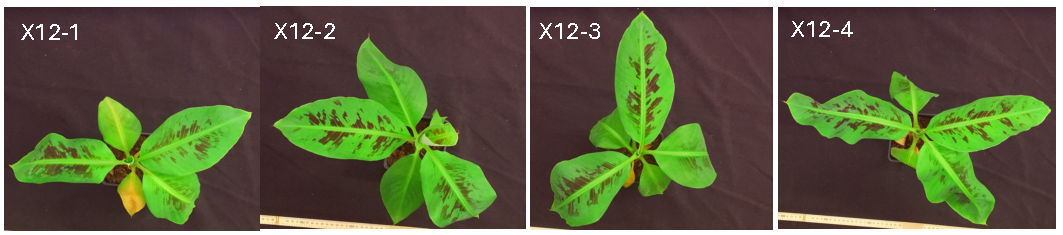
\includegraphics[width=\textwidth]{Figures/SecondTimePointXanthomonasBLQs.pdf}
    \caption{}
    \label{fig:XvmSecondTimeBLQs}
  \end{subfigure}
   \begin{subfigure}[b]{\textwidth}
    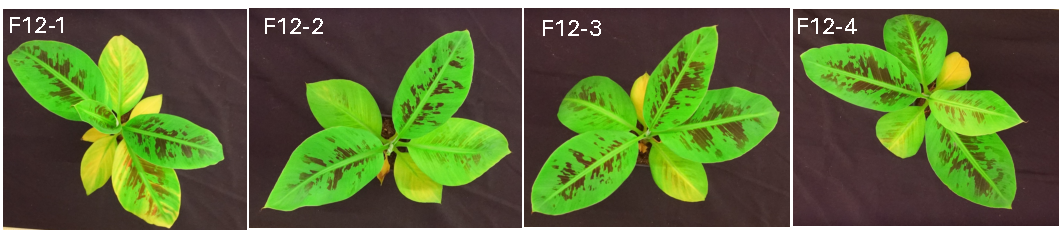
\includegraphics[width=\textwidth]{Figures/SecondTimePointFusariumBLQs.pdf}
    \caption{}
    \label{fig:FocSecondTimeBLQs}
  \end{subfigure}
     \begin{subfigure}[b]{\textwidth}
    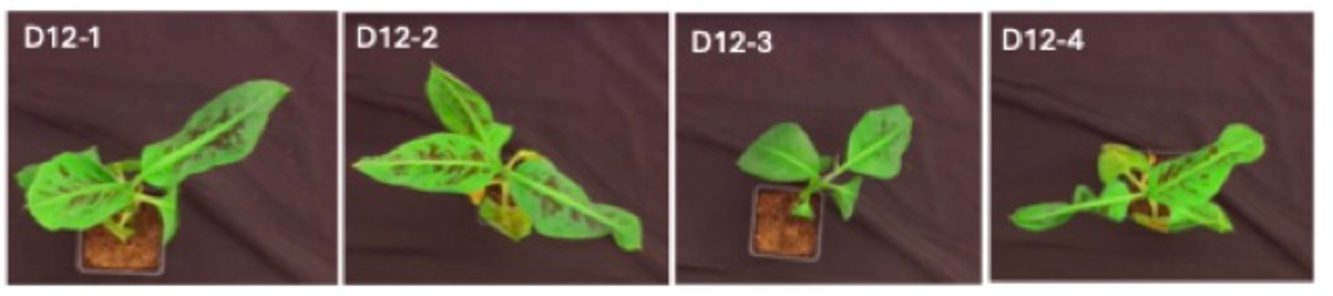
\includegraphics[width=\textwidth]{Figures/SecondTimePointDroughtBLQs.pdf}
    \caption{}
    \label{fig:DroSecondTimeBLQs}
  \end{subfigure}
     \begin{subfigure}[b]{\textwidth}
    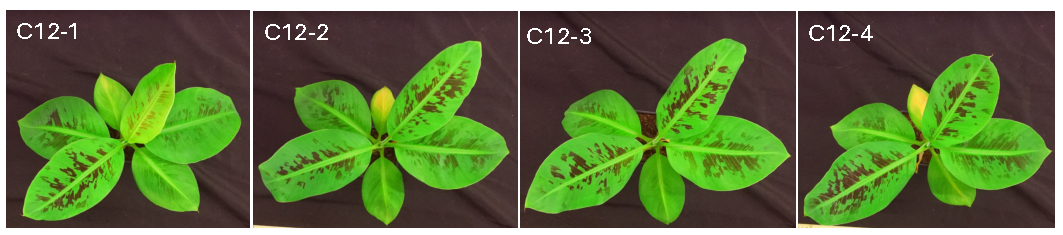
\includegraphics[width=\textwidth]{Figures/SecondTimePointControlBLQs.pdf}
    \caption{}
    \label{fig:ConSecondTimeBLQs}
  \end{subfigure}
  \caption[RGB images of 'Grande Naine' banana plants at the second sample time points.]{\textbf{RGB images of 'Grande Naine' banana plants at the second sample time points.}
  \textbf{\subref{fig:XvmSecondTimeBLQs}}) \acl{xvm}-inoculated plants at 10 \acl{dpi}.
  \textbf{\subref{fig:FocSecondTimeBLQs}}) \acl{Focub4}-inoculated plants at 18 \acl{dpi}.
  \textbf{\subref{fig:DroSecondTimeBLQs}}) Drought-stressed plants at 10, no-watering.
  \textbf{\subref{fig:ConSecondTimeBLQs}}) Mock-inoculated plants at 10 \ac{dpi}.
  Plant labels are provided in white text and correspond to sample labels used in \acl{um} analysis.
  }
  \label{fig:SecondTimePointSymptoms}
\end{figure}

\begin{figure}[ph!]
  \centering
  \begin{subfigure}[b]{\textwidth}
    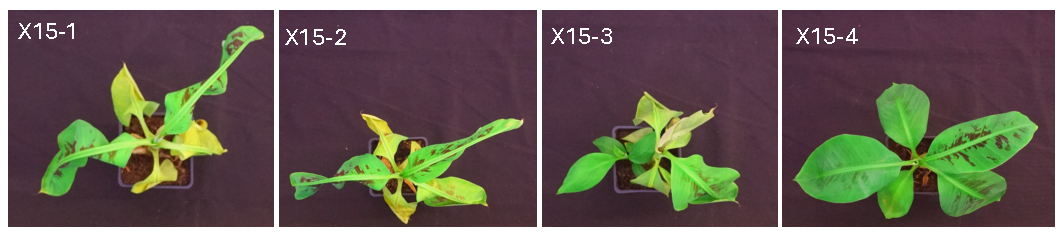
\includegraphics[width=\textwidth]{Figures/ThirdTimePointXanthomonasBLQs.pdf}
    \caption{}
    \label{fig:XvmThirdTimeBLQs}
  \end{subfigure}
   \begin{subfigure}[b]{\textwidth}
    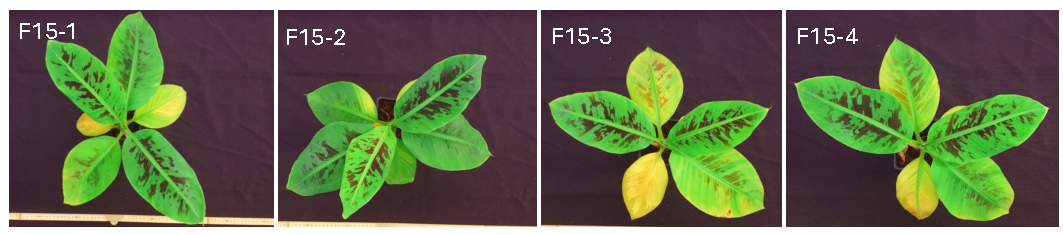
\includegraphics[width=\textwidth]{Figures/ThirdTimePointFusariumBLQs.pdf}
    \caption{}
    \label{fig:FocThirdTimeBLQs}
  \end{subfigure}
     \begin{subfigure}[b]{\textwidth}
    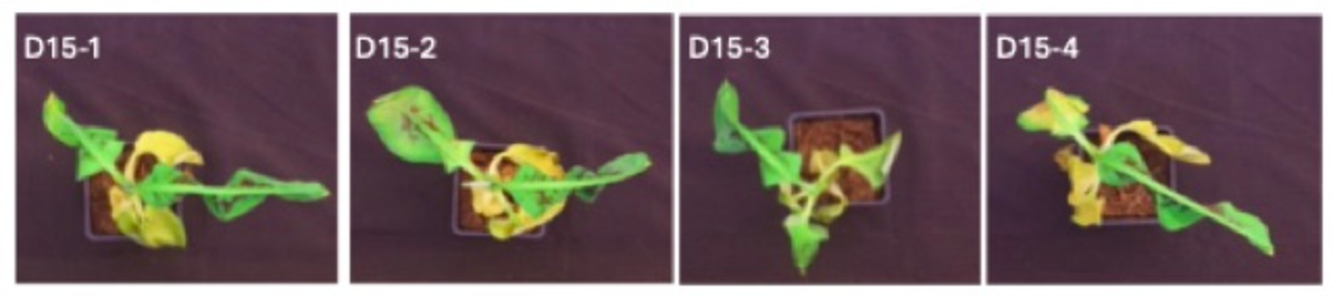
\includegraphics[width=\textwidth]{Figures/ThirdTimePointDroughtBLQs.pdf}
    \caption{}
    \label{fig:DroThirdTimeBLQs}
  \end{subfigure}
     \begin{subfigure}[b]{\textwidth}
    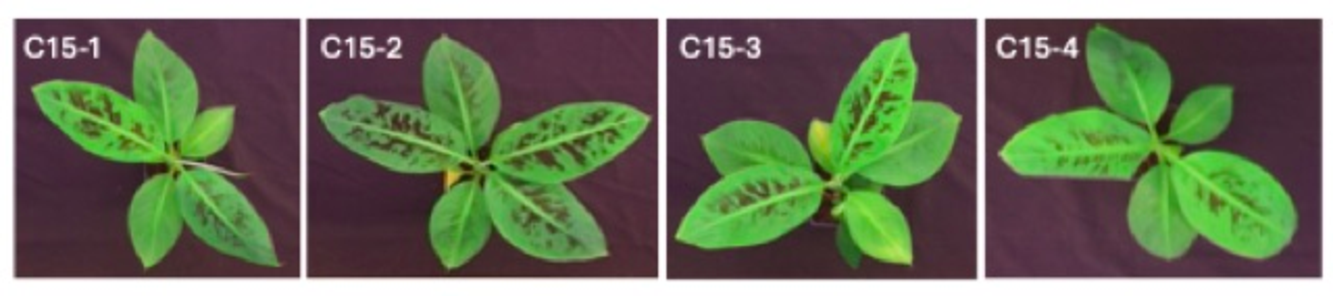
\includegraphics[width=\textwidth]{Figures/ThirdTimePointControlBLQs.pdf}
    \caption{}
    \label{fig:ConThirdTimeBLQs}
  \end{subfigure}
  \caption[RGB images of 'Grande Naine' banana plants at the third sample time points.]{\textbf{RGB images of 'Grande Naine' banana plants at the third sample time points.}
  \textbf{\subref{fig:XvmThirdTimeBLQs}}) \acl{xvm}-inoculated plants at 13 \acl{dpi}.
  \textbf{\subref{fig:FocThirdTimeBLQs}}) \acl{Focub4}-inoculated plants at 21 \acl{dpi}.
  \textbf{\subref{fig:DroThirdTimeBLQs}}) Drought-stressed plants at 13 days no-watering.
  \textbf{\subref{fig:ConThirdTimeBLQs}}) Mock-inoculated plants at 13 \ac{dpi}.
  Plant labels are provided in white text and correspond to sample labels used in \acl{um} analysis.
  }
  \label{fig:ThridTimePointSymptoms}
\end{figure}


\newpage
\begin{figure}[htp!]
    \centering
    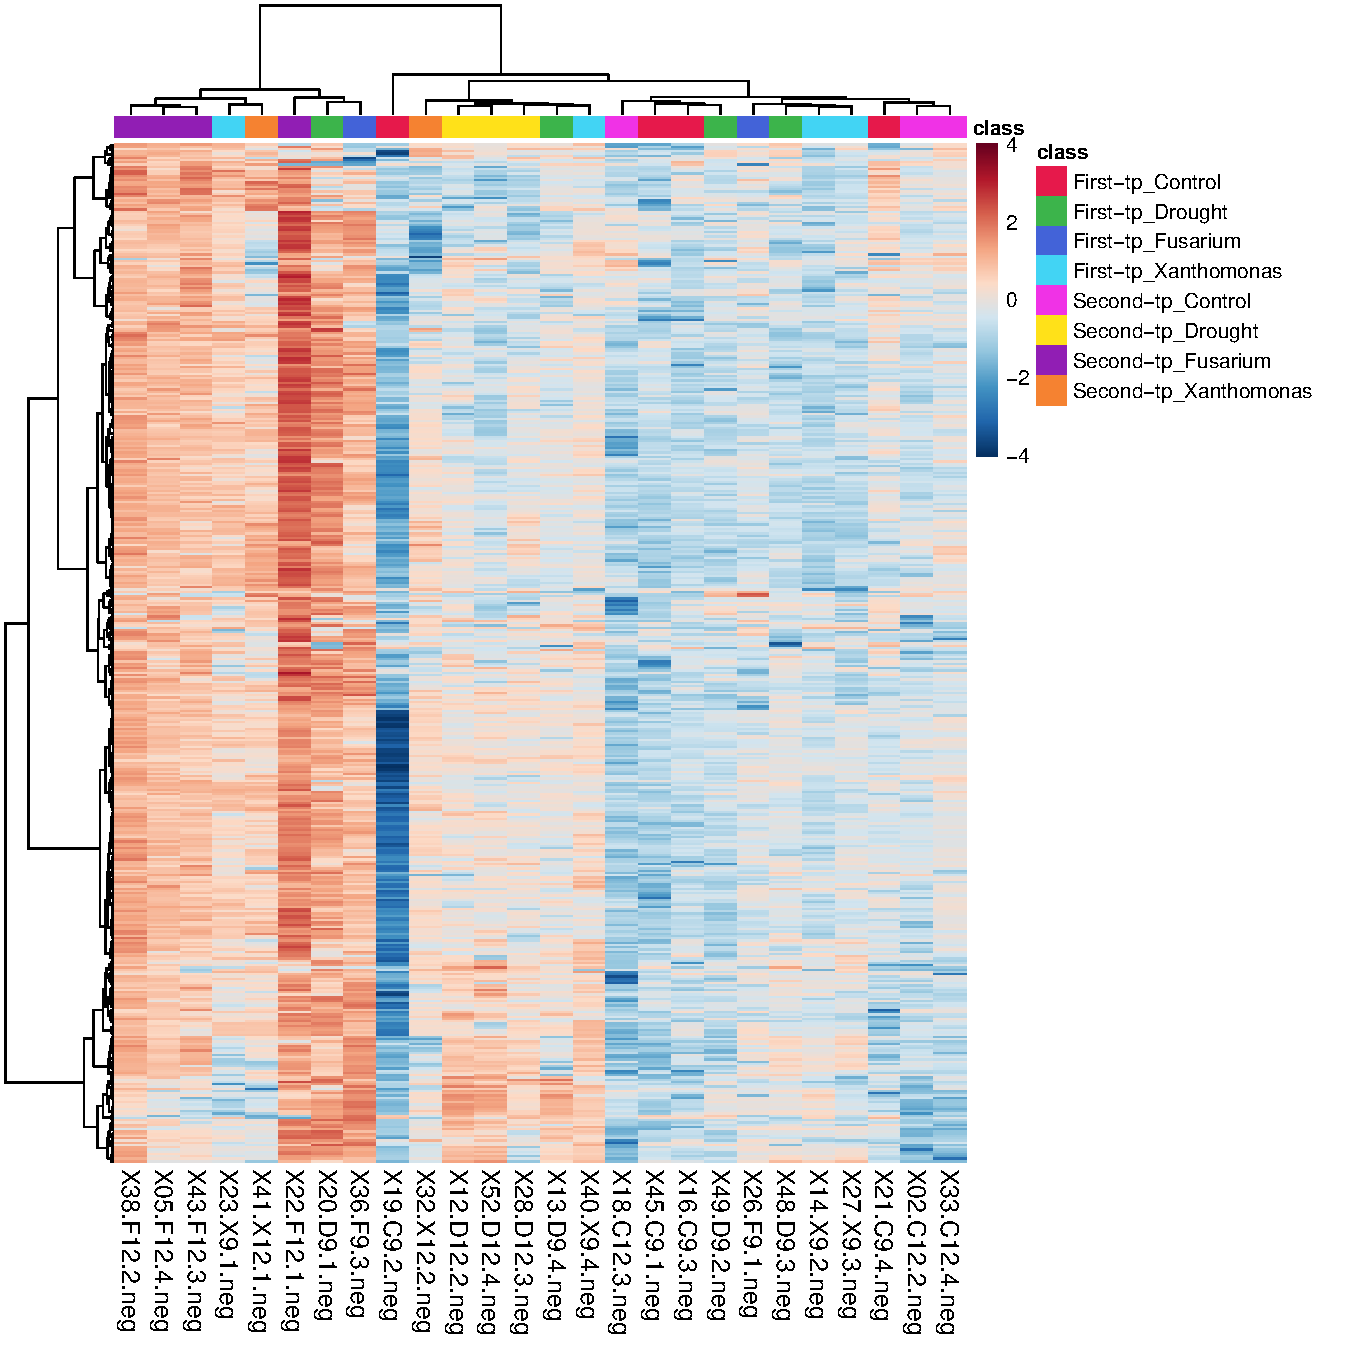
\includegraphics[width=\textwidth]{Appendices/Sig453FeaturesRedSamplesRedGroups.pdf}
    \caption[Heatmap showing hierarchical clustering of samples based on 453 normalised significant feature peak intensities (p ≤ 0.05) (negative mode)]{\textbf{Heatmap showing hierarchical clustering of samples based on 453 normalised significant feature peak intensities (p ≤ 0.05) (negative mode).} The distance measure was Euclidean and the ward.D algorithm was used for clustering. Class shows the treatment time and group. Value shows the normalised peak intensity. Values show normalised peak intensity. Features were normalised to the sodium formate \ch{Na(NaCOOH)3} adduct, log-transformed and scaled (Pareto scaling). Figure generated using MetaboAnalyst (v6.0).}
    \label{fig:Sig543FeaturesNegMode}
\end{figure}

\newpage
\begin{figure}[htp!]
    \centering
    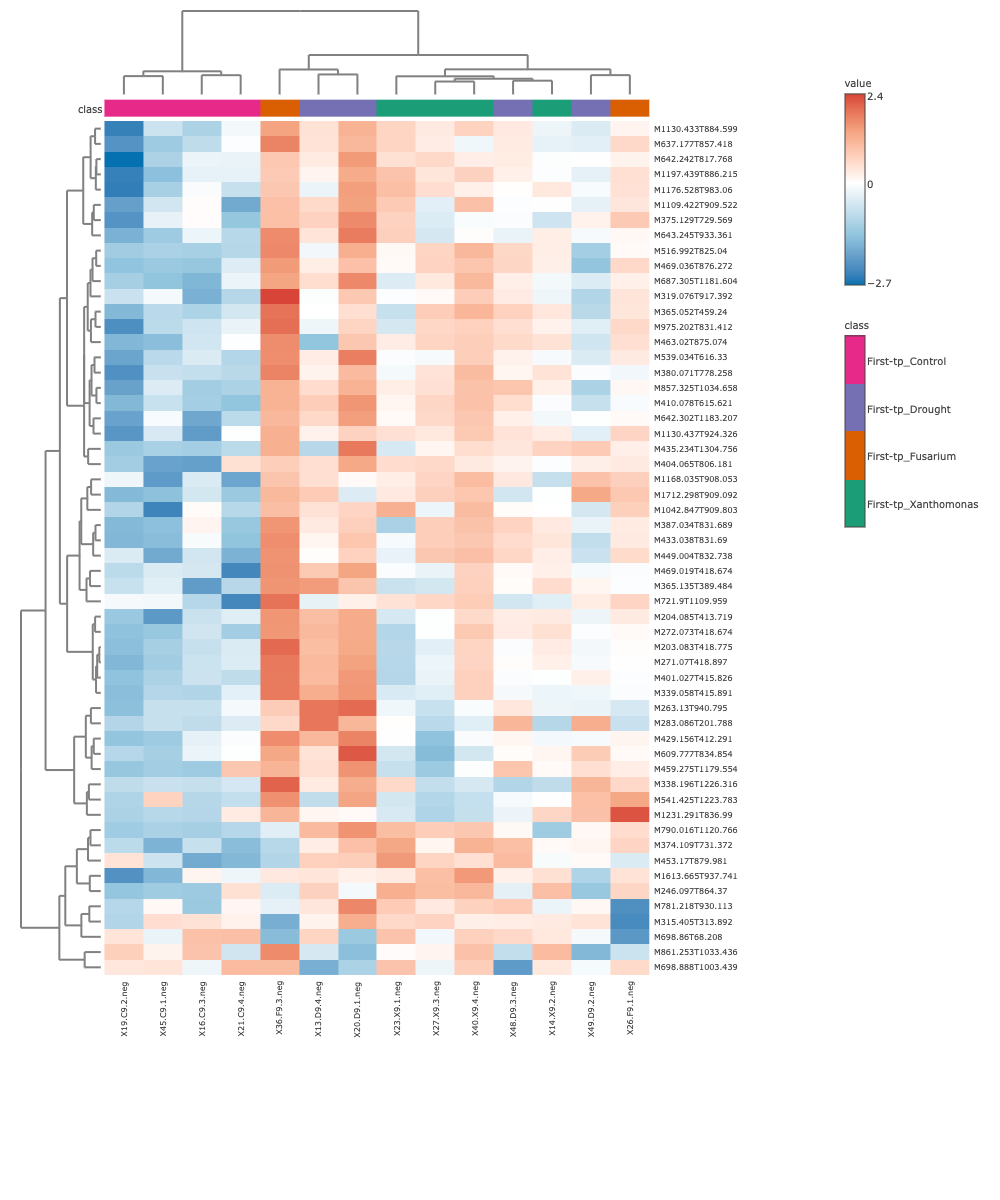
\includegraphics[width=\textwidth]{Appendices/Sig56FeaturesRedSamplesFirstTimePointOnly-ExcludingQCs.png}
    \caption[Heatmap showing hierarchical clustering of samples based on 56 normalised significant feature peak intensities (p ≤ 0.05) from the first time point (negative mode)]{\textbf{Heatmap showing hierarchical clustering of samples based on 56 normalised significant feature peak intensities (p ≤ 0.05) from the first time point (negative mode).} The distance measure was Euclidean and the ward.D algorithm was used for clustering. Class shows the treatment group. Value shows the normalised peak intensity. Values show normalised peak intensity. Features were normalised to the sodium formate \ch{Na(NaCOOH)3} adduct, log-transformed and scaled (Pareto scaling). Figure generated using MetaboAnalyst (v6.0).}
    \label{fig:Sig56FeaturesNegMode}
\end{figure}

\newpage
\begin{figure}[htp!]
    \centering
    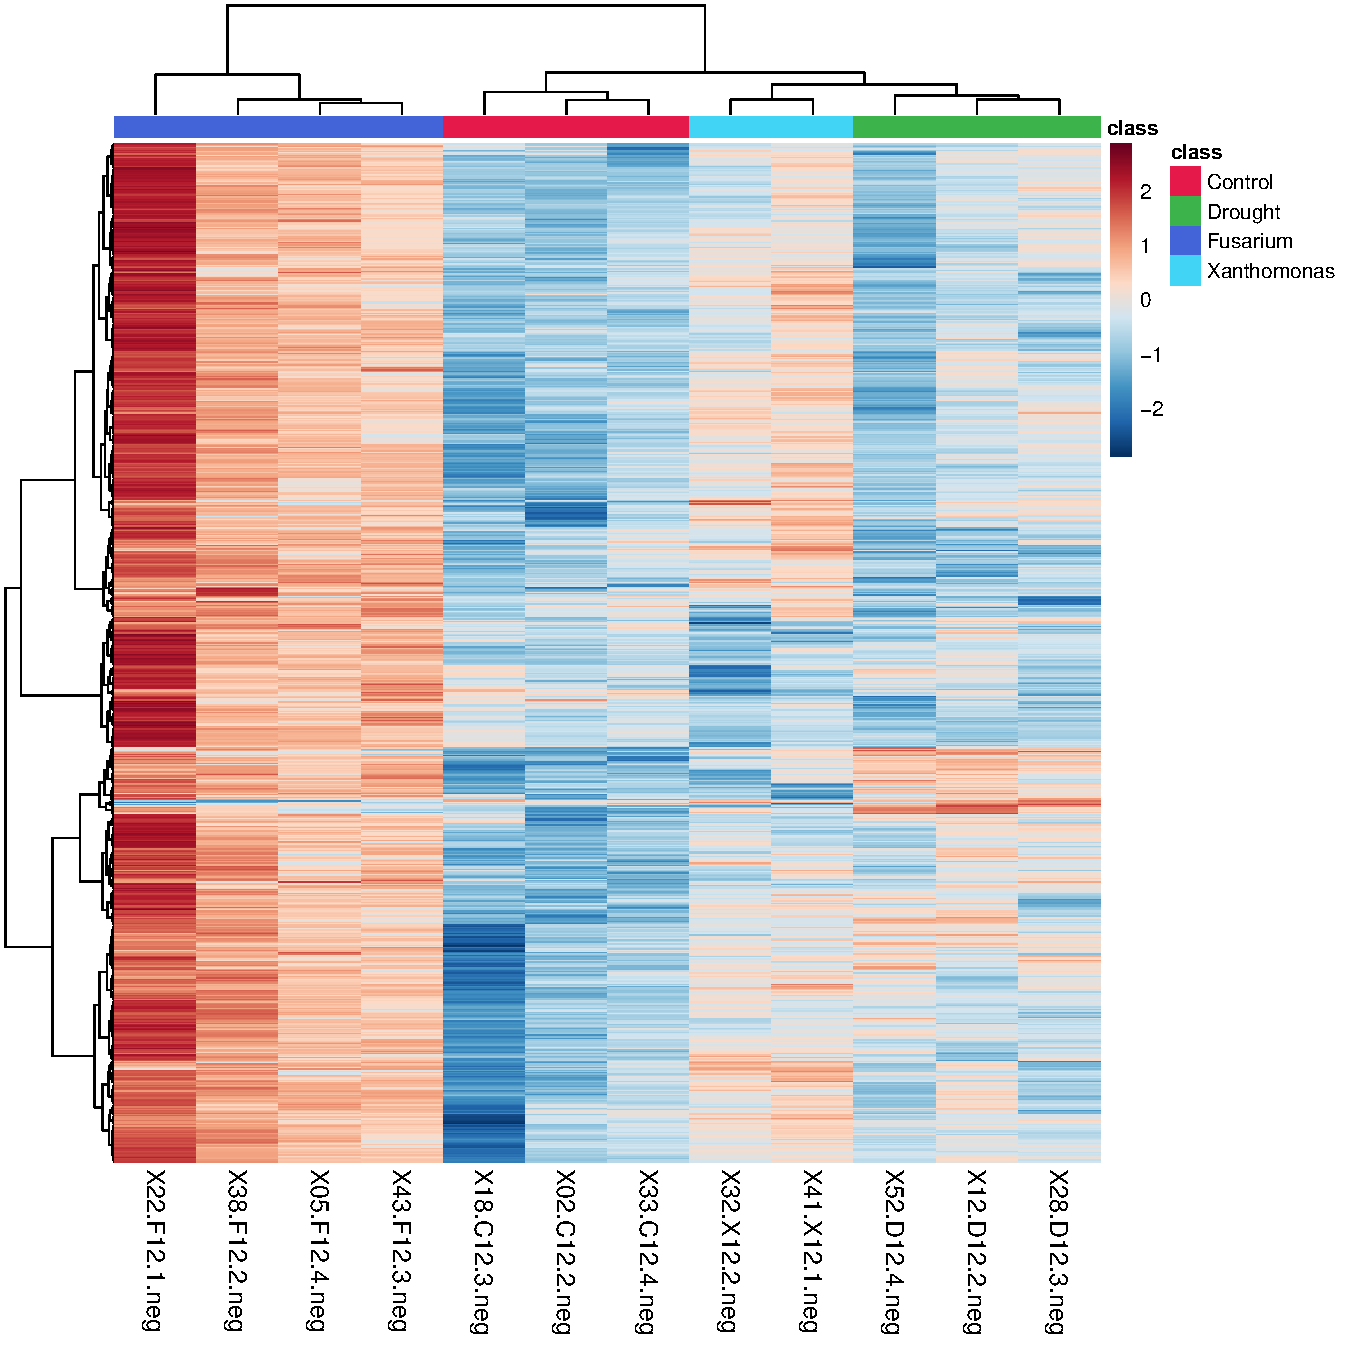
\includegraphics[width=\textwidth]{Appendices/RedSamplesSecondTimePoint-NonParametric-ExcludingQCs_heatmap_2_dpi72.pdf}
    \caption[Heatmap showing hierarchical clustering of samples based on 806 normalised significant feature peak intensities (p ≤ 0.05) from the first time point (negative mode)]{\textbf{Heatmap showing hierarchical clustering of samples based on 806 normalised significant feature peak intensities (p ≤ 0.05) (non-parametric ANOVA) from the first time point (negative mode).} The distance measure was Euclidean and the ward.D algorithm was used for clustering. Class shows the treatment group. Value shows the normalised peak intensity. Values show normalised peak intensity. Features were normalised to the sodium formate \ch{Na(NaCOOH)3} adduct, log-transformed and scaled (Pareto scaling). Figure generated using MetaboAnalyst (v6.0).}
    \label{fig:Sig806FeaturesNegMode}
\end{figure}